\documentclass[11pt,a4paper]{article}
\usepackage[T1]{fontenc}
\usepackage[utf8]{inputenc}
\usepackage{lmodern}
\usepackage{amsmath,amssymb,amsthm,mathtools,mathrsfs}
\usepackage{graphicx,float,xcolor,multicol}
\usepackage[shortlabels]{enumitem}
\usepackage[margin=27mm]{geometry}
\usepackage{microtype,needspace,placeins}
\usepackage{tikz,tikz-cd}
\usetikzlibrary{arrows.meta,calc,positioning,patterns,decorations.pathreplacing}
\usepackage[colorlinks=true,linkcolor=teal,urlcolor=teal,citecolor=teal]{hyperref}
\setlength{\parindent}{0pt}
\setlength{\parskip}{.6em}
\setcounter{secnumdepth}{0}
\allowdisplaybreaks
\raggedbottom
\providecommand{\cross}{\times}
\DeclareUnicodeCharacter{2020}{\ensuremath{\dagger}}
\DeclareMathOperator{\supp}{supp}
\DeclareMathOperator*{\esssup}{ess\,sup}
\providecommand{\chapter}{\section}
\newenvironment{tool}[2]{\subsection*{Tool #1 --- #2}}{}
\newcommand{\ToolRef}[1]{Tool #1}
\newcommand{\FigureTag}[2]{\textit{Figure #1}}
\newcommand{\Result}[1]{\subsection*{#1}}
\newcommand{\Application}[1]{\subsubsection*{Application\if\relax\detokenize{#1}\relax\else\space--- #1\fi}}
\newcommand{\ProofHeading}{\par\textit{Proof.}\space}
\newcommand{\ProofOf}[1]{\par\textit{Proof of #1.}\space}
\newcommand{\RemarkHeading}{\par\textbf{Remark.}\space}
\newcommand{\NoteHeading}{\par\textbf{Note.}\space}
\newcommand{\ExerciseHeading}{\par\textbf{Exercise.}\space}

% Rendering support only; mathematical text is in each independent post.
\usepackage{booktabs,array,longtable}
\definecolor{HandoutBlue}{HTML}{2F6690}
\definecolor{HandoutNavy}{HTML}{17365D}
\newtheorem{theorem}{Theorem}
\newtheorem{lemma}[theorem]{Lemma}
\newtheorem{proposition}[theorem]{Proposition}
\newtheorem{corollary}[theorem]{Corollary}
\newtheorem{conjecture}[theorem]{Conjecture}
\newtheorem{definition}{Definition}
\newtheorem{example}{Example}
\newtheorem{namedtoolcounter}{Tool}
\newenvironment{namedtool}[1]{\begin{namedtoolcounter}[#1]}{\end{namedtoolcounter}}
\newtheorem*{claim}{Claim}
\newtheorem*{remark}{Remark}
\newtheorem*{exercise}{Exercise}
\newtheorem*{question}{Question}
\newtheorem*{observation}{Observation}
\newcommand{\SourceChapter}[2]{\section*{#2}}
\newcommand{\Lecture}[2]{\section*{Lecture #1: #2}}
\newcommand{\unclear}[1]{\textit{[unclear: #1]}}
\newcommand{\sourcegap}{\textit{[unfinished in the source]}}
\DeclareMathOperator{\dist}{dist}
\DeclareMathOperator{\id}{id}
\DeclareMathOperator{\Hol}{Hol}
\DeclareMathOperator{\Per}{Per}
\DeclareMathOperator{\Fix}{Fix}
\DeclareMathOperator{\diam}{diam}
\DeclareMathOperator{\Var}{Var}
\DeclareMathOperator{\Leb}{Leb}
\DeclareMathOperator{\Hom}{Hom}
\DeclareMathOperator{\End}{End}
\DeclareMathOperator{\Ann}{Ann}
\DeclareMathOperator{\Spec}{Spec}
\DeclareMathOperator{\Max}{Max}
\DeclareMathOperator{\Ob}{Ob}
\DeclareMathOperator{\Tor}{Tor}
\DeclareMathOperator{\Ass}{Ass}
\DeclareMathOperator{\Mor}{Mor}
\DeclareMathOperator{\Fun}{Fun}
\DeclareMathOperator{\Nat}{Nat}
\DeclareMathOperator{\Cone}{Cone}
\DeclareMathOperator{\MCG}{MCG}
\DeclareMathOperator{\Aut}{Aut}
\DeclareMathOperator{\Deck}{Deck}
\DeclareMathOperator{\SL}{SL}
\DeclareMathOperator{\PSL}{PSL}
\DeclareMathOperator{\Area}{Area}
\DeclareMathOperator{\im}{im}
\DeclareMathOperator{\PSh}{PSh}
\newcommand{\CRing}{\mathsf{CRings}}
\newcommand{\AMod}{A\text{-}\mathsf{Mod}}
\newcommand{\Ab}{\mathsf{Ab}}
\newcommand{\Z}{\mathbb Z}
\newcommand{\Q}{\mathbb Q}
\newcommand{\R}{\mathbb R}
\newcommand{\C}{\mathbb C}
\newcommand{\N}{\mathbb N}
\newcommand{\kk}{\mathbb k}
\renewcommand{\aa}{\mathfrak a}
\newcommand{\bb}{\mathfrak b}
\newcommand{\pp}{\mathfrak p}
\newcommand{\qq}{\mathfrak q}
\newcommand{\mm}{\mathfrak m}
\newcommand{\nn}{\mathfrak n}
\newcommand{\rad}{\mathrm r}
\newcommand{\cat}[1]{\mathsf{#1}}
\setcounter{secnumdepth}{0}
\allowdisplaybreaks

\graphicspath{{figures/lemma-book/}}
\begin{document}
\section*{Puzzles, Surprises, and Marvellous Methods of Multiplication}
% BLOG-CONTENT-BEGIN
\setcounter{theorem}{44}\begin{lemma}[Check the hypotheses]
An elegant calculation is useful only after its assumptions have been checked.
\end{lemma}
The following example shows how an apparently perfect calculation can conceal a basic oversight.
Find $a^2+b^2+c^2$ where
$a^2+2b=6$, $b^2+4c=-7$, and $c^2+6a=-13$.
Adding gives
\begin{align*}
(a^2+2b)+(b^2+4c)+(c^2+6a)&=-14,\\
(a^2+6a)+(b^2+2b)+(c^2+4c)&=-14,\\
(a^2+6a+9)+(b^2+2b+1)+(c^2+4c+4)&=0,\\
(a+3)^2+(b+1)^2+(c+2)^2&=0.
\end{align*}
Thus $a=-3,b=-1,c=-2$, and $a^2+b^2+c^2=9+1+4=14$.
Notice that $a=-3,b=-1,c=-2$ do not satisfy the first and last equations.
The error was to assume, without checking, that a real solution exists.
Here is another example.
\paragraph{Leningrad Mathematical Olympiad.}
In triangle $ABC$, $\angle B=60^\circ$, $AD\perp BC$, and $CE\perp AB$.
Prove that the circumcentre of $ABC$ lies on the common bisector of $\angle AOE$ and $\angle COD$.
Here $O=AD\cap CE$.
Begin with the following figure.
% Source page 21 - left
Let $\omega$ be the circumcircle of triangle $AOC$, meeting the common bisector $\ell$ at $X$.
Then $AOXC$ is cyclic. Drop the perpendicular from $X$ to $AC$ at $M$.
We have
\begin{align*}
\angle DOE&=120^\circ=\angle AOC=\angle AXC,\\
\angle DOC&=\angle ABC=60^\circ=2\angle XOC,
\quad\text{so }\angle XOC=30^\circ,\\
\angle XOC&=\angle XAM=30^\circ=\pi/2-\angle AXM,
\quad\text{so }\angle AXM=60^\circ.
\end{align*}
Thus $\angle MXC=60^\circ=\angle AXM$, giving $\triangle AXM\cong\triangle CXM$ and $MA=MC$.
Therefore $XM$ is a perpendicular bisector.
Since $\angle AXC=120^\circ=2\angle ABC$, $X$ is the circumcentre, so the circumcentre lies on $\ell$.
\begin{figure}[H]\centering
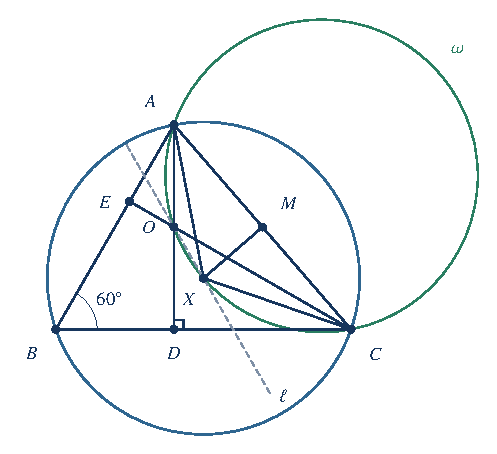
\includegraphics[width=.79\linewidth]{lb1-fig-15.pdf}
\FigureTag{LB1.15}{fig:lb1-15}
\end{figure}
The case $X=O$ is shown separately below.
\begin{figure}[H]\centering
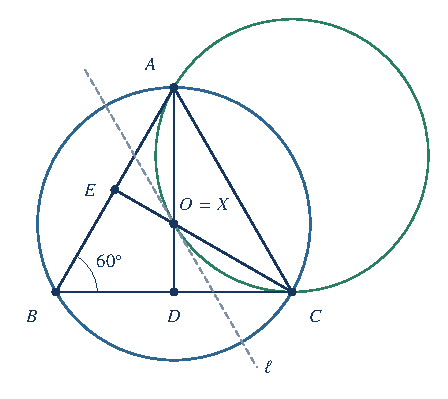
\includegraphics[width=.73\linewidth]{lb1-fig-16.pdf}
\FigureTag{LB1.16}{fig:lb1-16}
\end{figure}

\paragraph{Average speed.}
A plane travels from $A$ to $B$ at $160$ mph and returns from $B$ to $A$ at $240$ mph.
Find its average speed.
The usual temptation is $(160+240)/2=200$ mph, giving a wrong answer.
The two trips do not take the same time. If their common distance is $L$, then
$T_1=L/160$ and $T_2=L/240$.
The average time is $(T_1+T_2)/2$, while total time is
$T_1+T_2=L/160+L/240=L/96$.
Total distance is $2L$, so average speed is $2L/(L/96)=192$ mph.


\paragraph{Ramanujan's problem.}
Find $\sqrt{1+2\sqrt{1+3\sqrt{1+4\sqrt{1+5\sqrt{1+\cdots}}}}}$.
Use
\[
x+1=\sqrt{1+x(x+2)}
=\sqrt{1+x\sqrt{1+(x+1)(x+3)}}
=\sqrt{1+x\sqrt{1+(x+1)\sqrt{1+\cdots}}}.
\]
Put $x=2$.

Without calculating $\sqrt2$, show that $7/5$ is closer to it than $3/2$.
We do not know $\sqrt2$, but we do know $(\sqrt2)^2$.

\paragraph{A coordinate-geometry calculation.}
Given $\vec P(t)=A(\hat\imath\cos(kt)-\hat\jmath\sin(kt))$, determine the angle between $\vec P(t)$ and $\vec F(t)$, where $P(t)$ and $F(t)$ are momentum and force.
We have
\[\vec F(t)=\frac{dP(t)}{dt}=-Ak\sin(kt)\hat\imath-Ak\cos(kt)\hat\jmath
=\frac{\partial(A\cos(kt))}{\partial t}\hat\imath
-\frac{\partial(A\sin(kt))}{\partial t}\hat\jmath.\]
Plot the two vectors in the coordinate plane.
% Source page 40 - right
\begin{figure}[H]\centering
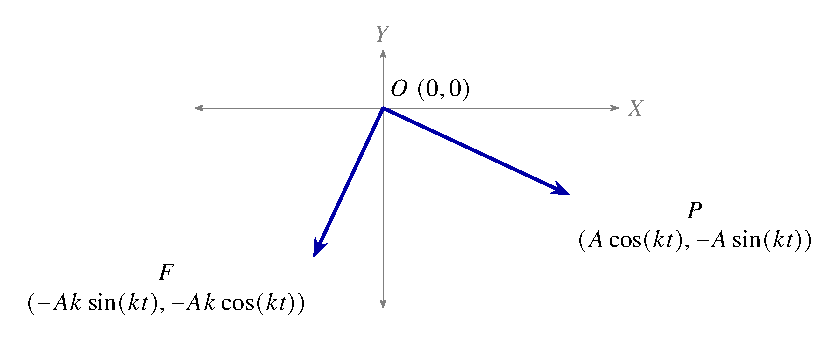
\includegraphics[width=.78\linewidth]{lb1-fig-20.pdf}
\FigureTag{LB1.20}{fig:lb1-20}
\end{figure}
\[
\begin{aligned}
FO&=\sqrt{A^2k^2\sin^2(kt)+A^2k^2\cos^2(kt)}=Ak,\\
PO&=\sqrt{A^2\cos^2(kt)+A^2\sin^2(kt)}=A,\\
FP&=\sqrt{A^2(\cos(kt)+k\sin(kt))^2+A^2(k\cos(kt)-\sin(kt))^2}
=A\sqrt{k^2+1}.
\end{aligned}
\]
We have $OF^2+OP^2=FP^2$, so $\angle FOP=\pi/2=90^\circ$. Q.E.D.!

You are not supposed to do these bullshits: just put $t=0$ in $P(t)$ and $F(t)$.
This gives $P(0)=A\hat\imath$ and $F(0)=-Ak\hat\jmath$.
$P$ is along $X$, and $F$ is along $-Y$, so $\angle FOP=\pi/2$. Q.E.D.!
Taken alone, this only checks the angle at $t=0$. For every $t$, however, the
same conclusion follows immediately from
\[
\vec P(t)\cdot\vec F(t)
=-A^2k\cos(kt)\sin(kt)+A^2k\sin(kt)\cos(kt)=0.
\]

You know what? You are not even supposed to play those dirty tricks.
For this circular motion, $\vec a\cdot\vec v=0$, $\vec F=m\vec a$, and
$\vec P=m\vec v$. Thus $\vec F\cdot\vec P=m^2\vec a\cdot\vec v=0$,
giving $\vec F\perp\vec P$. Another Q.E.D.! Enough!

% Source page 42 - left

\paragraph{British Mathematical Olympiad (2014).}
Prove that it is impossible to have a cuboid whose volume, surface area, and perimeter are numerically equal.
We have $V=lbh$, $S=2(lb+bh+hl)$, and $P=4(l+b+h)$.
It follows that
\[\frac1l+\frac1b+\frac1h=\frac12,
\qquad\frac1{lb}+\frac1{bh}+\frac1{hl}=\frac14.\]
Now
\[\left(\frac1l+\frac1b+\frac1h\right)^2
=\frac1{l^2}+\frac1{b^2}+\frac1{h^2}
+2\left(\frac1{lb}+\frac1{bh}+\frac1{hl}\right).\]
Thus $1/4-1/2=-1/4=1/l^2+1/b^2+1/h^2<0$, a contradiction.

\begin{quote}Common sense is like a deodorant: those who need it the most lack it!\end{quote}
\paragraph{1. Proportional angles.}\leavevmode\par
\begin{figure}[H]\centering
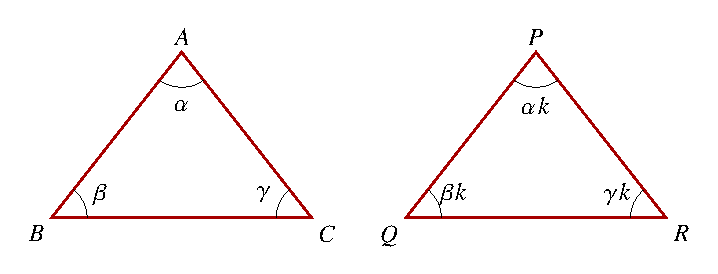
\includegraphics[width=.78\linewidth]{lb1-fig-30.pdf}
\FigureTag{LB1.30}{fig:lb1-30}
\end{figure}
Is $\triangle ABC\sim\triangle PQR$?
You might be wondering: if the sides are proportional, the triangles are similar, but what if the angles are proportional?
To tell you the reality, it's all a big dumbass!
Since $\alpha+\beta+\gamma=180^\circ$ and $\alpha k+\beta k+\gamma k=180^\circ$, we have $k=1$.
Thus the angles of $\triangle PQR$ are also $\alpha,\beta,\gamma$, so $\triangle ABC\sim\triangle PQR$.
Q.E.D.!
\paragraph{2. Solve the puzzle.}
$1=5$, $2=25$, $3=325$, $4=4325$. Then $5={}?$
\paragraph{3. Two digits.}
Construct the smallest possible integer using just two digits.
You know what? You can create a number as small as possible! But how?!

% Source page 54 - left
\paragraph{Answers.}
2. If $1=5$, then $5=1$. Q.E.D.!

The proposed answer is
\[
-\bigl[(9!!!!\cdots!)^{(9!!!!\cdots!)}\bigr].
\]
This is how it should be done!
As written, however, ``the smallest possible integer'' has no answer: allowing
unbounded factorials and exponents produces arbitrarily large negative integers.
\subsection{Mission impossible}
\paragraph{Compass-only midpoint.}
Construct the midpoint of a line segment without using a ruler, but only a compass!
I will not tell you exactly what I did. Go figure it out for yourself!
\begin{figure}[H]\centering
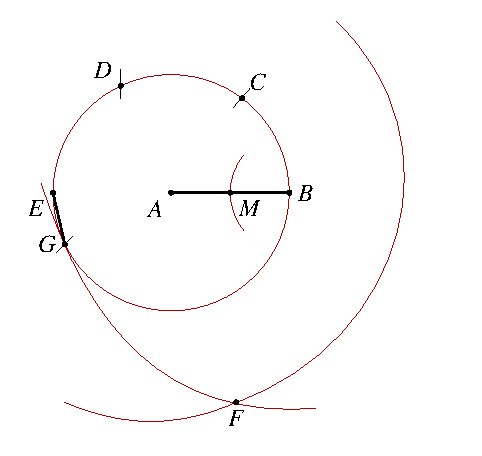
\includegraphics[width=.78\linewidth]{lb1-fig-31.pdf}
\FigureTag{LB1.31}{fig:lb1-31}
\end{figure}
\paragraph{Equilateral triangle.}
Inscribe an equilateral triangle inside an arbitrary triangle $ABC$. Challenge!
\subsection{Marvellous methods of multiplication: triple M}
\paragraph{The way Egyptian nerds did it!}
Suppose you want to multiply $11\times17$. They do the following:
\begin{center}
\begin{tabular}{lrrrrl}
Half sequence & $\boxed{11}$ & $\boxed5$ & $2$ & $\boxed1$ & $\lfloor n/2\rfloor$ in general\\
Double it & $17$ & $34$ & $68$ & $136$ & $2n$ in general
\end{tabular}
\end{center}
Identify the odd entries in the half sequence, and add the corresponding numbers from the double sequence.
We have $11\mapsto17$, $5\mapsto34$, and $1\mapsto136$, so the sum is $17+34+136=187=11\times17$.
Why does that bullshit work? Let's find out.
Suppose we are interested in the product $N\times M$.
\begin{center}
\begin{tabular}{lrrrrrrr}
Half & $N$ & $N/2$ & $N/4$ & $N/8$ & $N/16$ & $\cdots$ & $1$\\
Double & $M$ & $2M$ & $4M$ & $8M$ & $16M$ & $\cdots$ & $2^kM$
\end{tabular}
\end{center}
Express $N$ in binary: $N=2^{\alpha_1}+2^{\alpha_2}+\cdots+2^{\alpha_n}$.
For example, $11=2^3+2^1+2^0$.
The product $N\times M$ equals $2^{\alpha_1}M+\cdots+2^{\alpha_n}M$.
Each term $2^{\alpha_1}M,\ldots,2^{\alpha_n}M$ occurs in the double sequence.
Adding precisely those terms gives the product $N\times M$.
% Source page 55 - left
Now notice the half sequence: its $n$th entry is of the form
$\lfloor N/2^n\rfloor$. If $2^n$ is a part of the decomposition of $N$, then
\[
\begin{aligned}
\left\lfloor\frac N{2^n}\right\rfloor
&=\left\lfloor
\frac{2^{a_1}+2^{a_2}+\cdots+2^{a_j}+2^n
      +2^{b_1}+\cdots+2^{b_k}}{2^n}\right\rfloor\\
&=2^{a_1-n}+\cdots+2^{a_j-n}+1,
\end{aligned}
\]
where $a_i>n$ for all $i$, and $b_i<n$ for all $i$.
The powers $2^{a_i-n}$ are even, while the terms with exponents $b_i<n$
disappear upon taking the floor. Hence the displayed integer is odd.
Its parity is exactly the $n$th binary digit of $N$.
Thus $2^{\alpha_i}$ appears in the binary expansion of $N$ if and only if $\lfloor N/2^{\alpha_i}\rfloor$ is odd.
The corresponding double-sequence entry is $2^{\alpha_i}M$.
Adding all such terms gives $2^{\alpha_1}M+\cdots+2^{\alpha_n}M=N\times M$.
This proves the method.
\paragraph{Parabolic multiplication.}\leavevmode\par
\begin{figure}[H]\centering
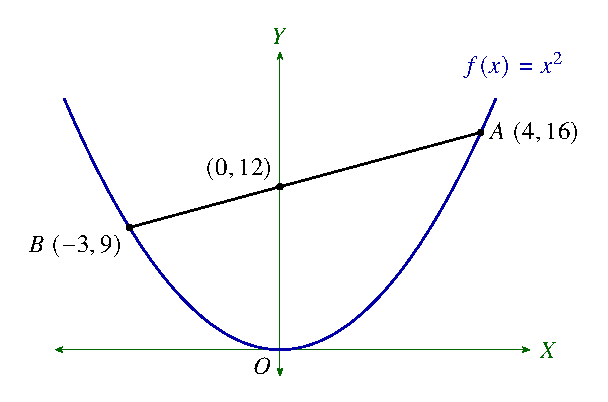
\includegraphics[width=.79\linewidth]{lb1-fig-32.pdf}
\FigureTag{LB1.32}{fig:lb1-32}
\end{figure}
Suppose you want $4\times3$. Take $A(4,16)$ and $B(-3,9)$.
Join $AB$: its intersection with the $Y$-axis gives the product!
The line through $(a,a^2)$ and $(-b,b^2)$ has slope $a-b$, so its value at $x=0$ is $a^2-a(a-b)=ab$.
% Source page 55 - right
\paragraph{A geometry problem leads to a continued fraction.}
$T_1$ is an isosceles triangle with circumcircle $K$.
Let $T_2$ be another isosceles triangle inscribed in $K$, whose base is one of the equal sides of $T_1$, and which overlaps the interior of $T_1$.
Similarly create $T_3$, and so on. Do the triangles $T_n$ approach an equilateral triangle as $n\to\infty$?
\begin{figure}[H]\centering
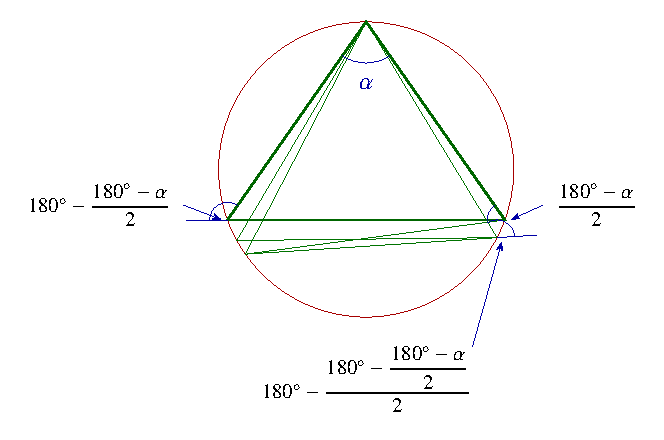
\includegraphics[width=.90\linewidth]{lb1-fig-33.pdf}
\FigureTag{LB1.33}{fig:lb1-33}
\end{figure}
The figure explains the vertex angles of $T_1,T_2,T_3,T_4$.
If $\theta_n$ is the vertex angle of $T_n$, then
\[\theta_{n+1}=\frac{180^\circ-\theta_n}{2}=90^\circ-\frac{\theta_n}{2}.\]
Hence
\[\theta_n=60^\circ+\left(-\frac12\right)^{n-1}(\theta_1-60^\circ),\]
and therefore $\theta_n\to60^\circ$. The triangles approach an equilateral triangle.

\paragraph{Out of the box.}
Place one of $+,-,\times,\div$ in each blank of $8\ \underline{\hspace{.5cm}}\ 8\ \underline{\hspace{.5cm}}\ 8=6$.
The answer, due to Shovan, is $(8\div8)+8=6$.
Reading the equation upside down turns the final $6$ into a $9$, and the equality becomes correct.

\paragraph{A trivial trick!}
Solve in real numbers:
\[
x=\sqrt{x+2\sqrt{x+2\sqrt{x+2\sqrt{x+2\sqrt{3x}}}}}.
\]
Put $T_x(t)=\sqrt{x+2t}$. The innermost radical is $T_x(x)$, and the
right-hand side is $T_x^{\circ5}(x)$. The map $T_x$ is increasing.
If $0<x<3$, then $T_x(x)=\sqrt{3x}>x$, so
$T_x^{\circ5}(x)>x$. If $x>3$, then $T_x(x)<x$, so
$T_x^{\circ5}(x)<x$. Hence a nonnegative solution must be $x=0$ or $x=3$,
and direct substitution shows that both work. Q.E.D.!

\paragraph{A complex-power puzzle.}
I remember asking this question; why do not you fiddle with it too?
Is $(-1)^\pi$ positive or negative? I hear you saying ``WTF!!!''
% Source page 18 - right
The answer was quite unexpected!
The value depends on the chosen branch of the logarithm. With the principal logarithm,
\[(-1)^\pi=\exp\bigl(\pi\operatorname{Log}(-1)\bigr)=e^{i\pi^2}
=\cos(\pi^2)+i\sin(\pi^2),\]
which is not real.

There is another proof. Represent $\pi=a/b$, where $a,b$ are not necessarily finite:
$\pi=(31415925\ldots)/10^\infty$. Since we cannot determine the last digit of $\pi$, we are done! Q.E.D.!
This formal calculation is not a proof, since $10^\infty$ is not a number and
exponentiation by a non-integer must first be defined by choosing a logarithm
branch; it is precisely that choice which the principal-logarithm calculation
above makes.
% BLOG-CONTENT-END
\end{document}
